% Исследовательская часть
\section{Исследовательская часть}

\hspace{1.25cm}
Для рассмотрения числа сравнений в зависимости от индекса на котором находится элемент для линейного и бинарного поисков элементов в массиве были собранны данные и составлены следующие гистограммы: для линейного поиска (см. рисунок~\ref{fig:bar_graph_linear}), для бинарного (см. рисунок~\ref{fig:bar_graph_binary}) и отсортированный по возрастанию числа сравнений для бинарного (см. рисунок~\ref{fig:bar_graph_binary_sort}). Алгоритмы запускались на массиве длиной 50, элементы которого соответствуют индексам и ищутся один за другим с шагом 1.

Замеры были проведены на процессоре 13-го поколения Intel(R) Core(TM) i5-
13500H с тактовой частотой 2.60 ГГц, оперативная память 16,0 ГБ, тип системы 64-
разрядная операционная система, процессор x64, версия Python 3.11.9.

\begin{figure}[H]
    \centering
    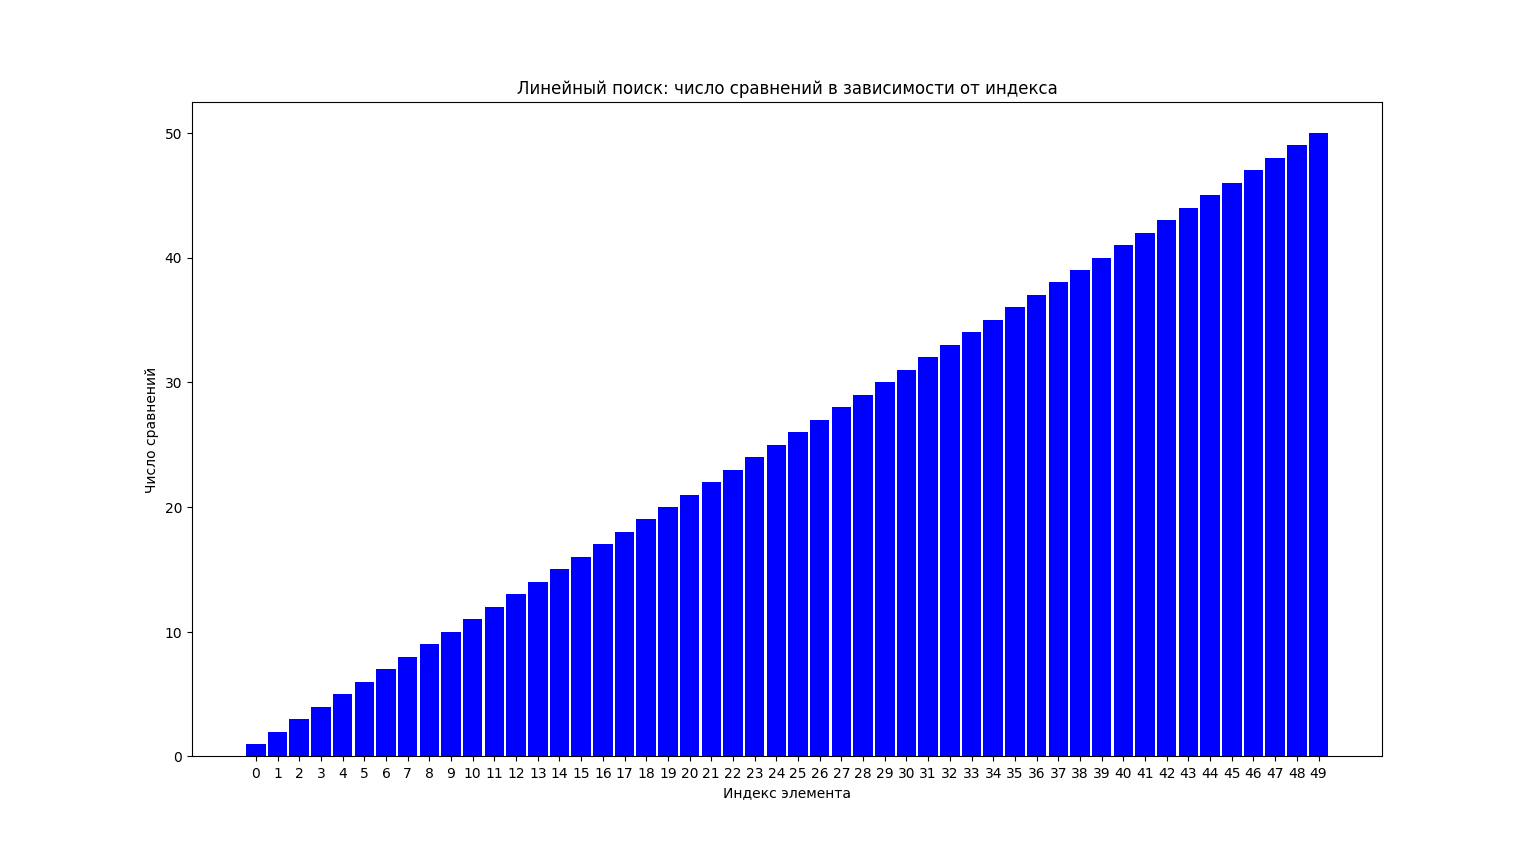
\includegraphics[width=1\textwidth]{img/bar_graph_linear.png}
    \caption{Гистограмма числа сравнений в зависимости от индекса на котором находится элемент для линейного поиска}
    \label{fig:bar_graph_linear} % Метка для ссылки на картинку
\end{figure}

\begin{figure}[H]
    \centering
    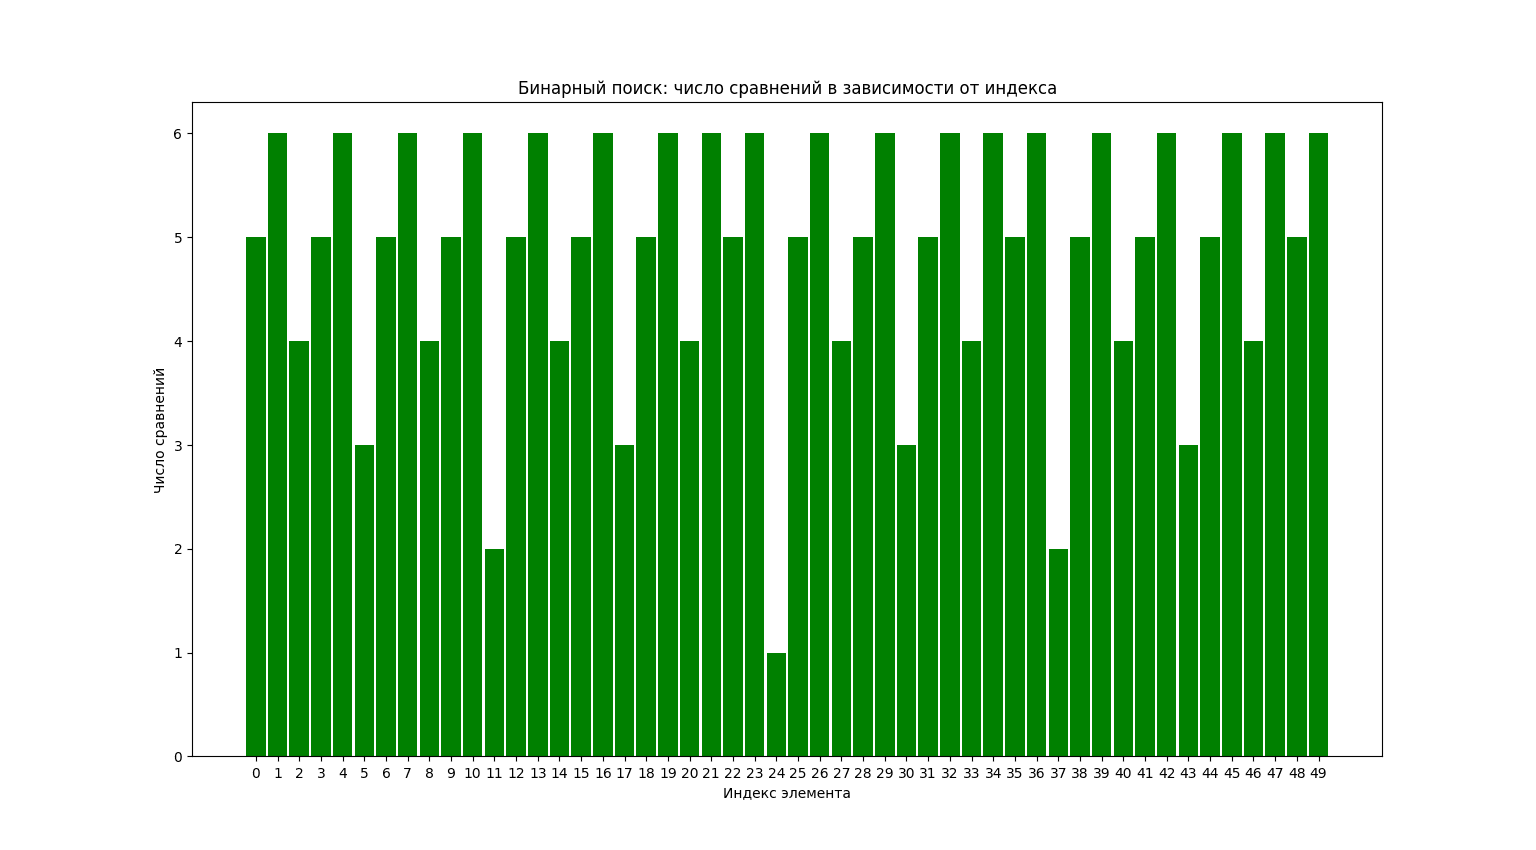
\includegraphics[width=1\textwidth]{img/bar_graph_binary.png}
    \caption{Гистограмма числа сравнений в зависимости от индекса на котором находится элемент для бинарного поиска}
    \label{fig:bar_graph_binary} % Метка для ссылки на картинку
\end{figure}

\begin{figure}[H]
    \centering
    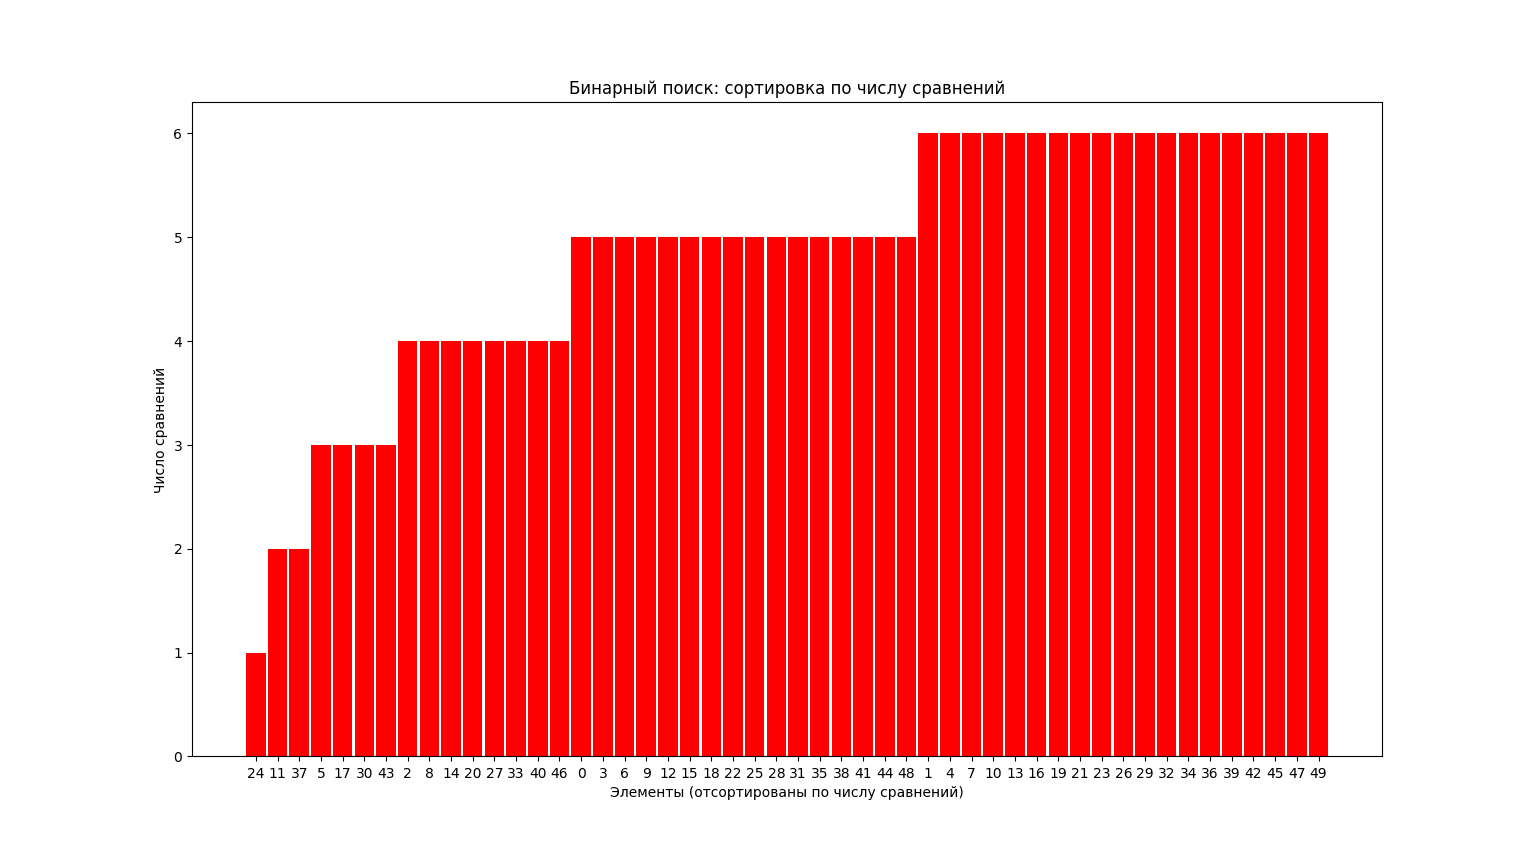
\includegraphics[width=1\textwidth]{img/bar_graph_binary_sort.png}
    \caption{Гистограмма числа сравнений в зависимости от индекса на котором находится элемент для бинарного поиска (отсортированная по возрастанию числа сравнений)}
    \label{fig:bar_graph_binary_sort} % Метка для ссылки на картинку
\end{figure}

\subsection*{Вывод}

\subsubsection*{Линейный поиск}

\hspace{1.25cm}
При линейном поиске сравнение производится последовательно от первого элемента до того, который совпадет с искомым значением. Число сравнений зависит от того, где находится искомый элемент:

\begin{enumerate}
    \item Если элемент находится на первом индексе, будет сделано 1 сравнение.
    \item Если на втором, то 2 сравнения и так далее.
    \item Если элемент отсутствует, требуется сравнить все 50 элементов.
\end{enumerate}

Таким образом, для элемента на индексе \(i\) число сравнений равно \(i + 1\).

\subsubsection*{Бинарный поиск}

\hspace{1.25cm}
При бинарном поиске массив делится на две части, и продолжается поиск в соответствующей половине, в зависимости от того, меньше или больше искомое значение среднего элемента. Число сравнений можно оценить как логарифм числа элементов массива:

\begin{equation}
\text{Число сравнений} \approx \log_2(n)
\end{equation}

где \(n\) — текущее количество элементов в части массива, где продолжается поиск.

Для массива из 50 элементов число сравнений для поиска элемента на разных индексах будет следующим:

число шагов при бинарном поиске для массива из 50 элементов — это округлённое значение $log_2(50)$, что примерно равно 6. Таким образом, бинарный поиск сделает около 6 сравнений для нахождения элемента.

\subsubsection*{Сравнение по индексам:}

\textbf{Линейный поиск:}
\begin{enumerate}
    \item Элемент на индексе 0: 1 сравнение.
    \item Элемент на индексе 1: 2 сравнения.
    \item Элемент на индексе 25: 26 сравнений.
    \item Элемент на индексе 49: 50 сравнений.
\end{enumerate}

\textbf{Бинарный поиск:}
Независимо от того, где находится элемент, максимальное количество сравнений не превысит 6 для массива из 50 элементов.

\subsubsection*{Вывод}

\hspace{1.25cm}
Линейный поиск имеет линейную сложность \(O(n)\), и число сравнений прямо зависит от позиции элемента. Бинарный поиск имеет логарифмическую сложность \(O(\log n)\) и обеспечивает гораздо меньшее число сравнений, особенно для элементов, находящихся ближе к концу массива, однако он работает только на отсортированных массивах, а сортировка может компенсировать выигрыш от более быстрого поиска.

\newpage